\documentclass[12pt]{article}


\usepackage[utf8]{inputenc}
\usepackage{cite}
\usepackage{algorithm}
\usepackage{amsmath}
\usepackage{algpseudocode}
\usepackage{lmodern}
\usepackage{microtype}
\usepackage{amsmath}
\usepackage{mathrsfs}
\usepackage{mathtools}
\usepackage{xcolor}
\usepackage{ulem}
\usepackage{graphicx}
\usepackage{float}
\usepackage{subfigure}
\usepackage[hyphens]{url}
\usepackage{setspace}
\usepackage{titlesec}
\usepackage[title]{appendix}


%\title{Automatic light dimmer}
\title{%
  \Huge Smart Alcohol Detector}
\author{Pena Benafa\\pena.benafa@stud.hshl.de\\
  \large Hardware Engineering Lab\\
  \large Summer Semester 2021}
\date{July 2021}


\onehalfspacing
\titlespacing*{\section}
{0pt}{5.5ex plus 1ex minus .2ex}{4.3ex plus .2ex}
\titlespacing*{\subsection}
{0pt}{5.5ex plus 1ex minus .2ex}{4.3ex plus .2ex}

\begin{document}


\maketitle
\begin{figure}[htbp]
\centering{
\includegraphics[scale=0.1]{figures/2000px-HSHL-Logo.svg.png}}

\label{fig}
\end{figure}

\begin{abstract}
   According to alcoholrehabguide, alcohol-related injuries have caused over 5.2 million people to die worldwide each year. \cite{a1}. In Germany, over a couple of months, there has been increased car crashes that result in severe injuries or even death due to drink-driving. The German Traffic Safety Council has sponsored several studies on the general prohibition of alcohol for driving a car \cite{a2}. Safety personnel on the roadside play a role in controlling the accident due to drink-driving using an alcohol detector, but this act is not efficient. This is because these personnel can't test all drivers using the road. A cheap, easy to install and use alcohol detector has been proposed in this report. The smart alcohol detector is a device that should be installed on modern cars. This will reduce road accidents drastically and further improve smart cars developed. The alcohol detector installed in cars will work in a way that before the car starts, an alcohol test must be initiated, and if the result is passed, the car can start otherwise, a display on the LCD will be alcohol detected car won't start. SAD uses a mechanism to detect the presence of alcohol from the user's breath.
\end{abstract}

\newpage
\tableofcontents
\newpage
\section{Field}

\section{Background}
One of the worst actions drivers can do on the road is Drink-driving. Intoxication can significantly impact a driver's decision-making, cognitive ability, car function and vision. 
Yet, as dangerous as this is, many people engage in drink-driving probably out of fun or ignorance. Unfortunately, drink-driving leads to fatal injuries or even death.
According to Parker Alexander, in the top 5 causes of car accidents, intoxication is the number one \cite{a3}. Early detection of alcohol can reduce road accidents to a significant level. However, this can be possible if alcohol detectors are installed in modern cars. This will prevent the car from starting whenever alcohol is detected from the driver's breath.  This project seeks to propose a system that will eliminate one of the causes of road accidents and further make modern cars smart vehicles.
\section{Summary of Invention}
This report looks at one of the significant causes of road accidents and how to control it using a device installed in cars. In addition, the report shows the design and implementation of the detector system. The device uses a microcontroller, FPGA and a sensor to detect alcohol levels in a driver body.
%
%Technical Problems
%


\section{Technical Problem}
Drunk while driving places oneself and other road users at risk. Alcohol has been a factor in traffic deaths over the years. Although security personnel has made an effort to control those driving
under the influence of alcohol, technology stops drivers from moving a vehicle when impaired could prevent fatal accidents. According to a report from Insurance Institute for Highway 
Safety in the US, a crash data in which high alcohol level was detected in the blood of at least one driver involved in a car crash \cite{a4}.

%
%Solution to problem
%



\section{Solution to Problem}
There are currently several proposed solutions to reduce drink-driving, such as licence suspension or revocation, licence plate confiscation, vehicle impoundment, increased penalties for drink-driving,
required alcohol education, and expanded use of designated drivers \cite{a5}. However, the effective prevention I will propose is the installation of an alcohol detector device in vehicles. Before the car starts, the driver has to test to determine alcohol in the body. If the level is high, the vehicle won't start.
%
%Advantageous Effects of Invention
%



\section{Advantageous Effects of Invention}
The component in the system that detects alcohol is called MQ3 alcohol sensor. The sensor uses SnO2(stannic oxide) material. In fresh air, the material offers low conductivity.
Whenever alcohol gas is present in the system, the conductivity of MQ3 sensor increases; that is, the resistance of the alcohol sensor reduces when concentration increases. An analog is rendered such a sound from a buzzer.

Below are some listed benefits of alcohol sensor

   1. The sensor is at a lower price.

   2. The stability level is high.
   
   3. The sensor has a good sensitivity response time.
   
   4. It is simple to install, and the drive circuit use is not complicated.
   
   5. It can be used to control drunk ness as well as protect properties from unwanted access.

\section{Brief Description of Drawings}
The block and schematic diagram in the figure below consists of the FPGA, which has a microprocessor. The microprocessor is a 32-bit soft core processor, and it can be programmed with c language. The microprocessor has an inbuilt driver. These drivers enable digital to analog conversion and analog to digital conversion. On the block diagram, the LCD is a 20by2 display unit. It outputs the system state and anytime. A variable resistor is attached to the LCD to control brightness.
There are four LEDs in the system, and each of them has its own functional indication. At the initial state, the yellow LEDs is displayed. This indicates that the system is in an idle state. The LED switch from yellow to blue whenever the test button is pressed. If alcohol is detected after the test taken, the LED switches to red; otherwise, it is green, indicating no alcohol detected, and the car start is enabled. The buzzer is an output device that uses a digital to analog converter to output sound. The sound from the buzzer indicates alcohol in the system. The push-button is used whenever the test is taken. The button and the temperature sensor function simultaneously. The temperature sensor compares the previous temperature of the car before the button was pressed and the temperature of the car after the button was pressed. The alcohol sensor consists of an MQ3 sensor. The sensor is used to detect alcohol from the user's breath. Whenever the conductivity of the MQ3 sensor increases, the buzzer will sound, a red LED will display, and the car state will be disabled. This is an indication that alcohol is detected. The JTAG is an interface whereby the FPGA can be programmed, while the SRAM is a memory used to save the program in the FPGA during run time.

In the VHDL code diagram below, it consists of a clock (clk) which runs continuously. Below it is a reset state. At first, the reset is will be in reset state for 1 clock cycle, and it operates in an active high reset. That is, whenever it is high, it reset the system. Btn1 is the button state. This indicates that alcohol testing is taking place when it is high. The alcohol level state is a 2 bit wide, and it encodes the state of the alcohol. That is, 00 means nothing is taking place or idle, 01 means when alcohol is detected and 10 when no alcohol is detected. The green simulation shows that when on high, no alcohol is detected and the car state will be activated. The yellow light when on high indicates the system is in reset state. The blue LED indicates the system is in test state when the btn1 is pressed. The red LED indicate detection of alcohol and this will be on high. The car start state is a 2 bit wide. Unless no alcohol detected, the car state will always remain deactivated.

\section{Industrial Applicability}
Alcohol detector can be applicable in different areas. Alcohol sensors can be used to analyse temperatures ranging from -10 °C to 50 °C. The alcohol sensor is highly sensitive to the detection of smoke, smoke and petrol in industrial fuels\cite{a8}.
Alcohol detector can be used in the car industry. This will be less cheap but of great advantage because so many lives can be saved.
Another application of alcohol detector is in work place or in areas where alcohol is prohibited. Also, in developed countries like Germany where the age restriction to alcohol is 18 and above, this can be used to detect alcohol in any minor consuming alcohol.

\section{Conclusion}
In this project, I have demonstrated that to develop a technology that can measure accurately a driver’s BAC. The use of VHDL to simulate the functionality of the technology was successful.

\newpage
\section{Citation List}
\listoffigures
\section{Patent Literature}
\section{Non-Patent Literature}
\cite{a9}
\cite{a10}
\bibliographystyle{plain}
\bibliography{non-patent}

\clearpage
\pagenumbering{arabic}% resets `page` counter to 1
\renewcommand*{\thepage}{A\arabic{page}}
\begin{appendices}
\section{Some Notation}

\begin{figure}[h]
    \centering
    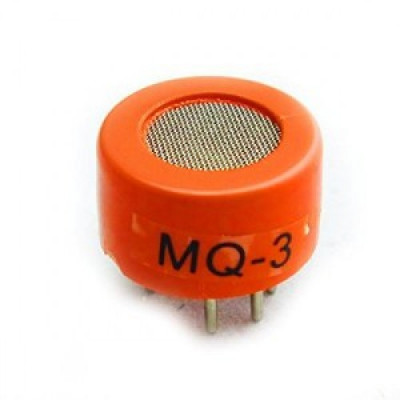
\includegraphics[width=0.48\textwidth]{HEL_template/figures/mq3-gas.jpg}
    \caption{MQ3 alcohol sensor \cite{img1}}
    \label{fig:alcohol sensor}
\end{figure}

\begin{figure}[h]
    \centering
    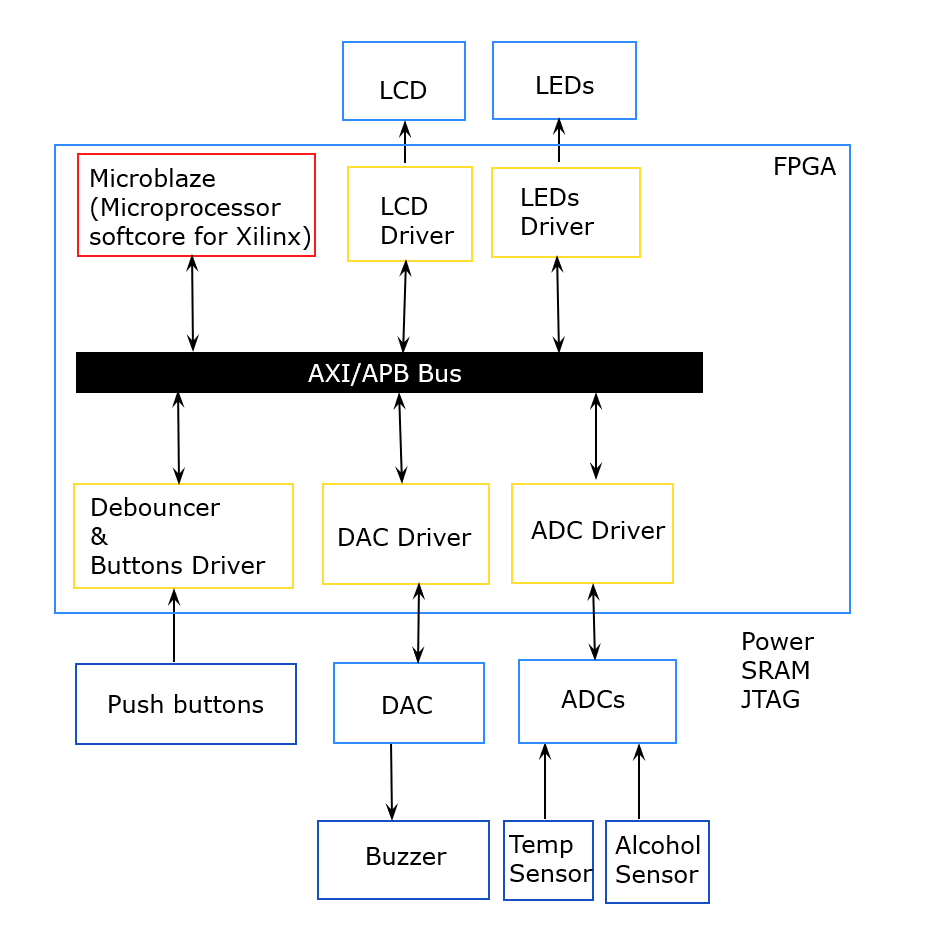
\includegraphics[width=0.75\textwidth]{HEL_template/figures/Block Diagram.png}
    \caption{System block diagram}
    \label{fig:block diagram}
\end{figure}

\begin{figure}[h]
    \centering
    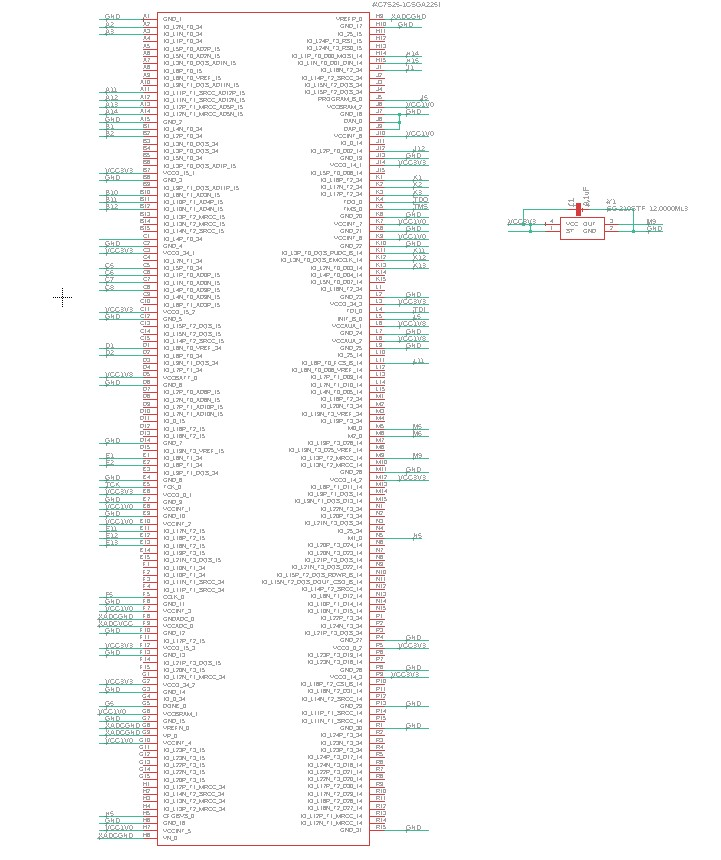
\includegraphics[width=0.75\textwidth]{HEL_template/figures/sheet1.jpg}
    \caption{FGPA Schematic Diagram}
    \label{fig:FGPA Schematic Diagram}
\end{figure}

\begin{figure}[h]
    \centering
    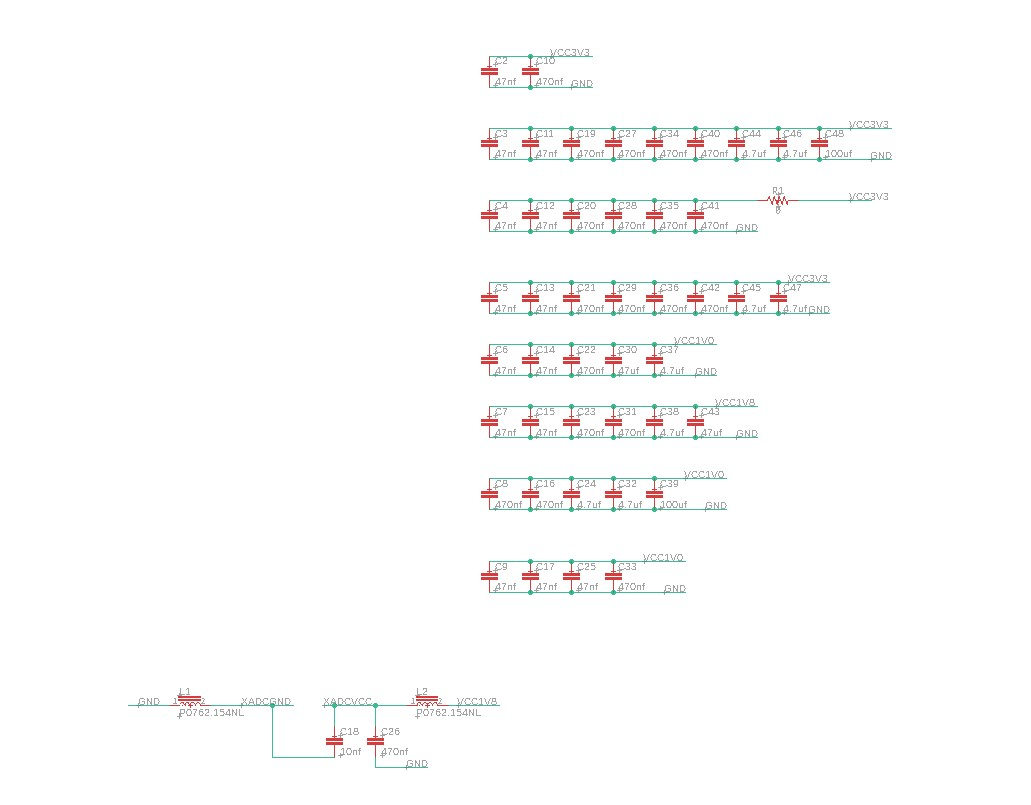
\includegraphics[width=0.75\textwidth]{HEL_template/figures/sheet2.jpg}
    \caption{ADC Schematic Diagram}
    \label{fig:Schematic Diagram}
\end{figure}

\begin{figure}[h]
    \centering
    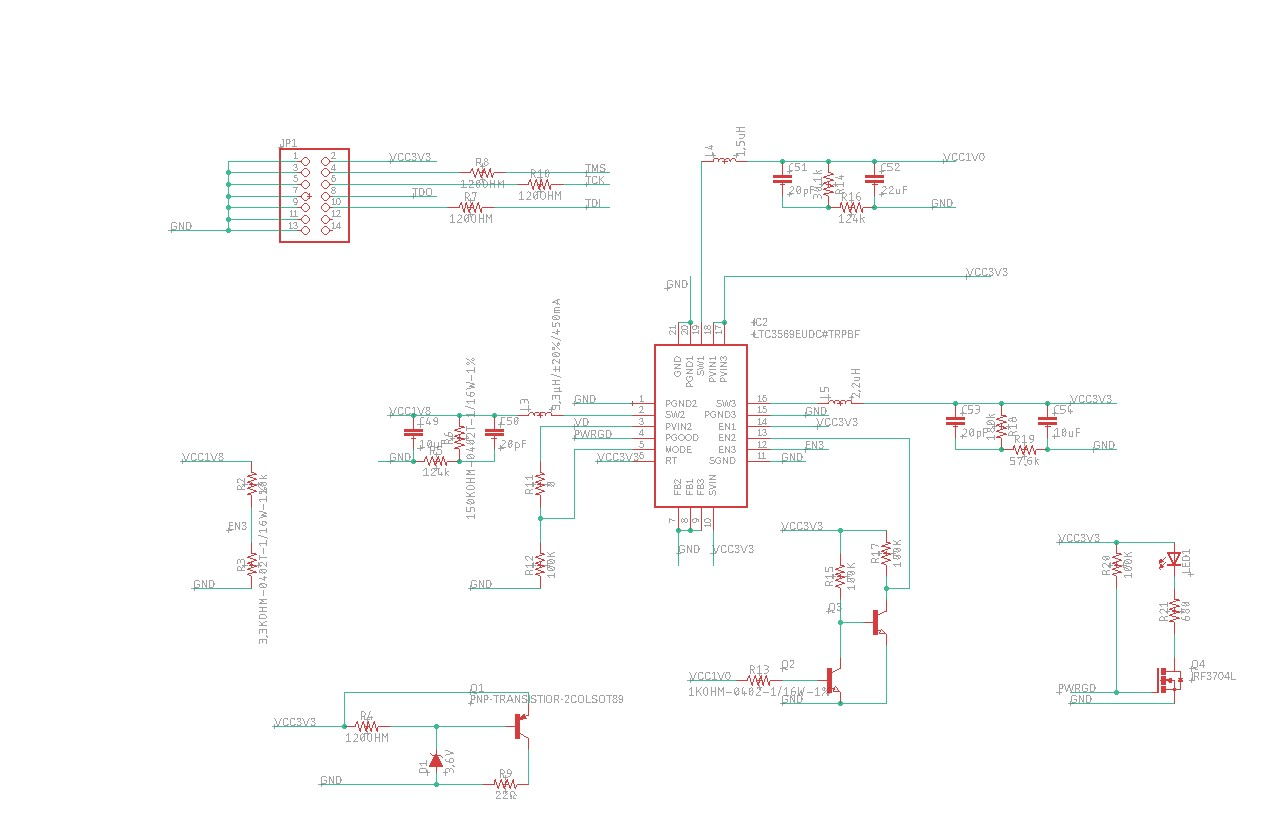
\includegraphics[width=0.75\textwidth]{HEL_template/figures/sheet3.jpg}
    \caption{Power converter Schematic Diagram}
    \label{fig:Power converter Schematic Diagram}
\end{figure}

\begin{figure}[h]
    \centering
    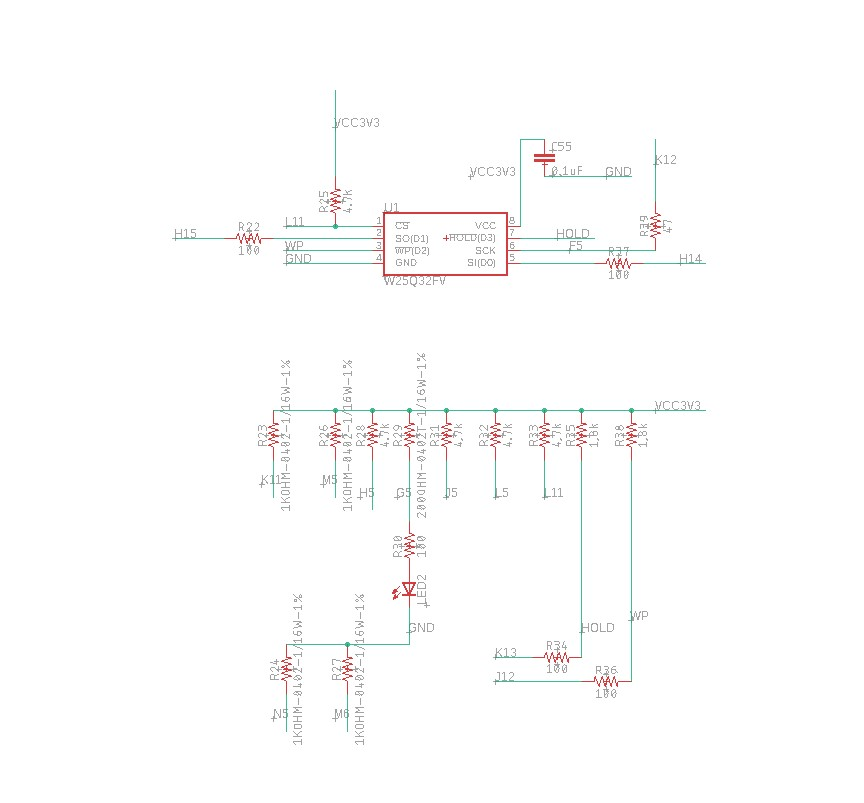
\includegraphics[width=0.75\textwidth]{HEL_template/figures/sheet4.jpg}
    \caption{SRAM Schematic Diagram}
    \label{fig:SRAM Schematic Diagram}
\end{figure}

\begin{figure}[h]
    \centering
    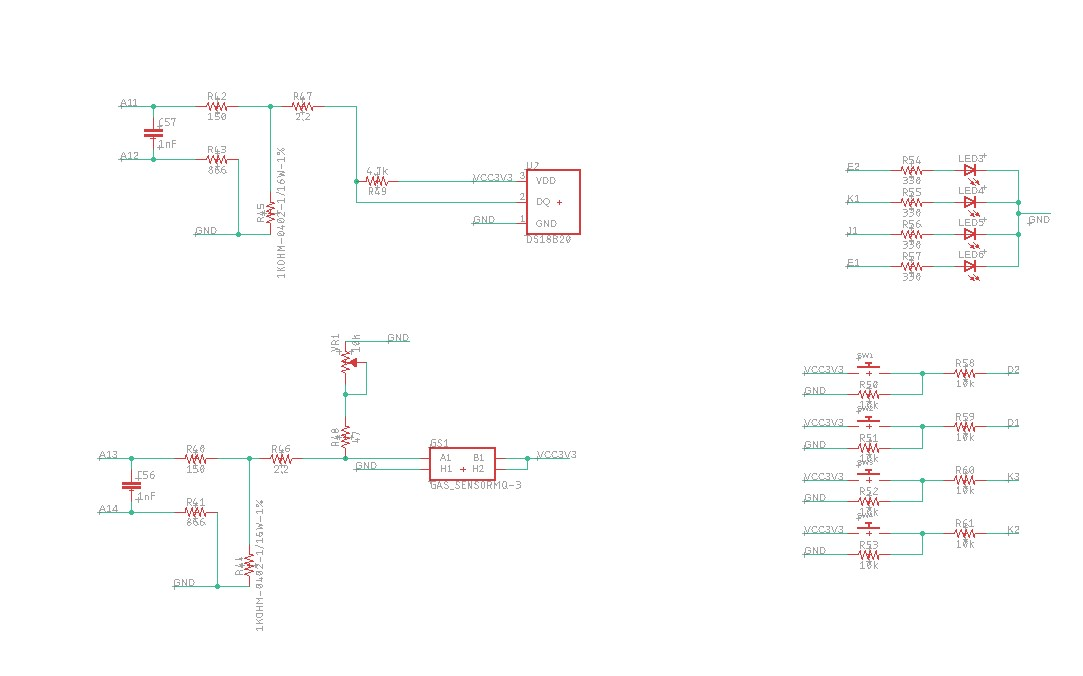
\includegraphics[width=0.75\textwidth]{HEL_template/figures/sheet5.jpg}
    \caption{Peripheral Schematic Diagram}
    \label{fig:Peripheral Schematic Diagram}
\end{figure}

\begin{figure}[h]
    \centering
    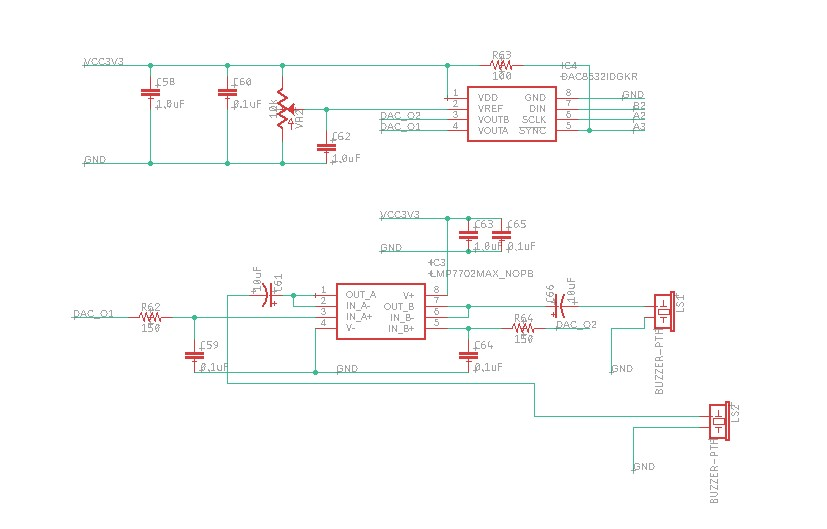
\includegraphics[width=0.75\textwidth]{HEL_template/figures/sheet6.jpg}
    \caption{DAC and amplifier Schematic Diagram}
    \label{fig:DAC and amplifier Schematic Diagram}
\end{figure}

\begin{figure}[h]
    \centering
    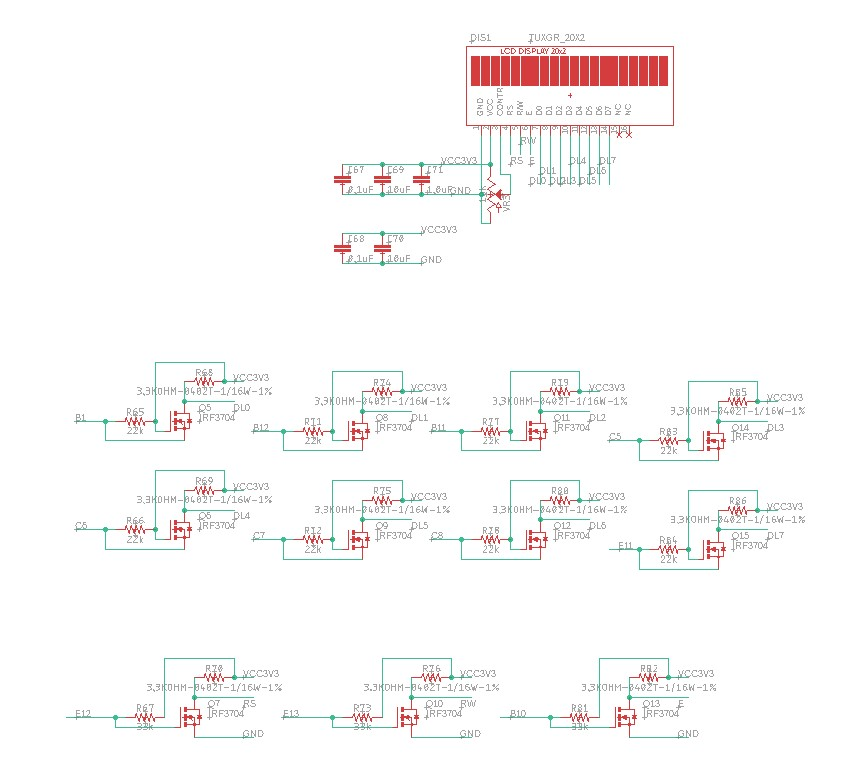
\includegraphics[width=0.75\textwidth]{HEL_template/figures/sheet7.jpg}
    \caption{LCD Schematic Diagram}
    \label{fig:LCD Schematic Diagram}
\end{figure}

\begin{figure}[h]
    \centering
    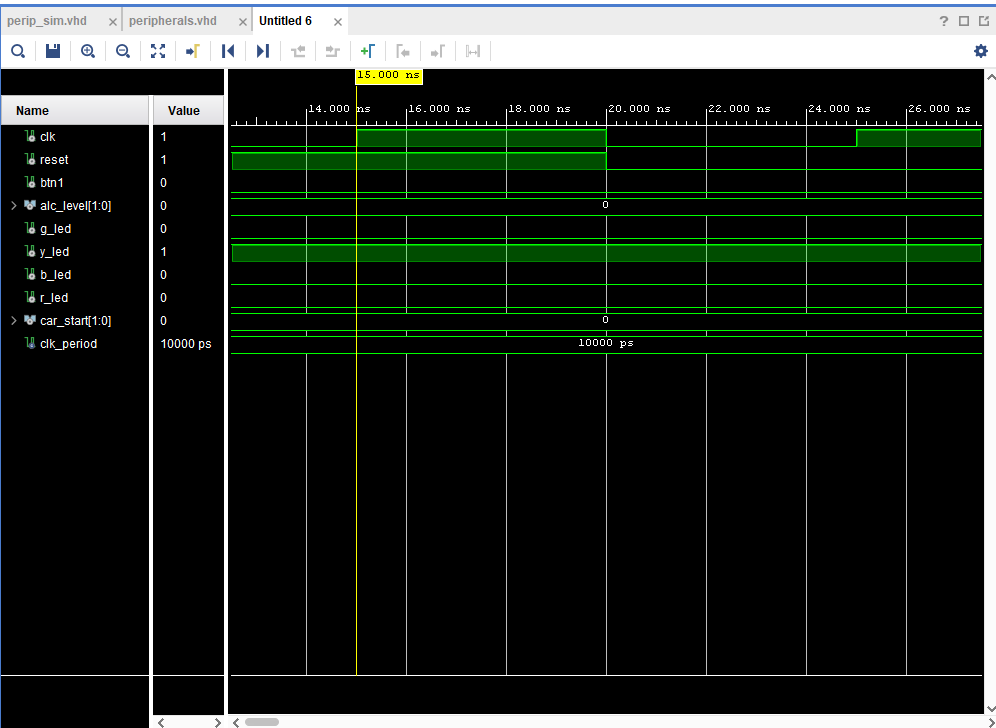
\includegraphics[width=0.75\textwidth]{HEL_template/figures/VHDL.png}
    \caption{VHDL code Diagram}
    \label{fig:VHDL code Diagram}
\end{figure}

\section{Some More Notation}
\end{appendices}

\end{document}
